\documentclass[a4paper,11pt]{article}
\usepackage[english]{babel}
\usepackage[T1]{fontenc}
\usepackage{fancyhdr}
\usepackage{graphicx}
\usepackage{a4wide}
\usepackage{numprint}
\usepackage{url}
\usepackage{cite}
\usepackage{multirow}
\usepackage{moreverb}
\usepackage{lastpage}
\usepackage{enumerate}
\pagestyle{fancy}

\author{Viktor Collin \\ <\url{vcollin@kth.se}> \\ 19880316-0277 \and Simon \"{O}sterman \\ <\url{simost@kth.se}> \\ 19880205-0156}
\title{\textbf{DH2323 Computer Graphics with Interaction \\ Lab 1 : Star field}}

\fancyhead[L]{\textbf{DH2323 : Lab 1} }
\fancyhead[R]{Viktor Collin \& Simon \"{O}sterman : Page \thepage }
\fancyfoot{}{}

\begin{document}
\maketitle
\begin{center}
Total pages: \pageref{LastPage}
\end{center}
\thispagestyle{empty}

\clearpage
\setcounter{page}{1}
\section*{Introduction}
This lab focuses on getting to know the basics of graphics programming such as the 
environments, libraries and simple algorithms to get started. After getting the environment running, the assignment is to write two programs; one in 2D and one in 3D. Below those two are explained in detail. 

\section{Interpolation}
\subsection{Assignment}
The assignment here is basically to get SDL running and to linearly interpolate between pixels on the screen to create a 2D-image.

\subsection{Method}
We started by defining the colors on the four corners of the screen. Next, we interpolate vertically between the lower and upper left and right corners. When we have the borders, we interpolate horizontally to achieve the image required. 

\subsection{Result}
After getting the environment and libraries up and running, we did not really encounter any problems doing this assignment. The task was pretty straight-forward and was a good introduction to the area of graphics programming. After implementing the program, the output produced was as in figure \ref{fig1}.
\begin{figure}[h!]
	\centering
	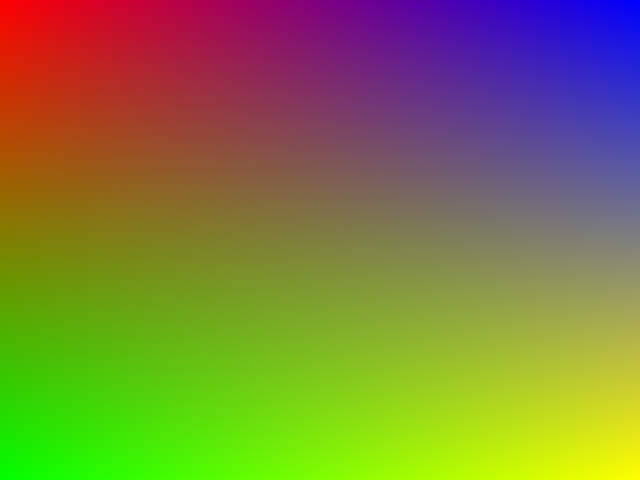
\includegraphics[width=0.75\linewidth]{screenshot1.png}
	\caption{Final output}
	\label{fig1}
\end{figure}

\clearpage
\section{Starfield}
\subsection{Assignment}
The second part of the lab is to create something called the star field effect. The star field effect is basically points which moves toward the camera in real-time. This creates the 3D illusion of moving forward through space.
\subsection{Method}
At first, the goal was simply to be able to spread the stars on our screen to get something that resembles a sky with a lot of stars. Once we got that done, the next task was to get the stars moving. The movement should only be along the z-axis but since we wanted a 3D-effect, some calculations was needed to realistically project the 3D-points onto a 2D-canvas. The next part of the implementation was to get the fading effect working. To keep the stars coming towards the camera we relocate the stars going out of the canvas to the back again. To avoid the effect of stars popping up out of nowhere we then make them fade instead of being full bright. Finally, as an inprovment, we made the stars have ''tails'' visualizing the speed they (or the camera) are traveling by and showing the projection of the distance recently travelled. 

\subsection{Result}
We did not have much trouble doing this part of the lab either. While there was a lot more math involved than in the first assignment, it was still pretty straight-forward to implement. The only real problem we encountered was our stars moving away from us rather than coming towards us which was required. The error was (of course) that we added instead of subtracted the z-value difference of the stars on each update.

Below is the output from the different stages of completion of our program:
\begin{figure}[h!]
	\centering
	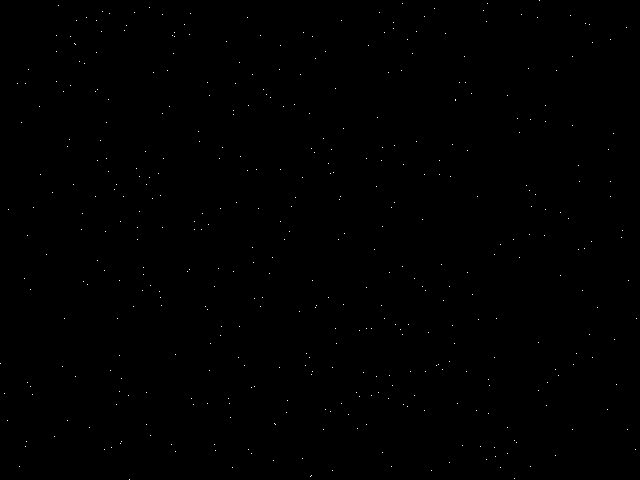
\includegraphics[width=0.7\linewidth]{screenshot2.png}
	\caption{Initial output}
	\label{fig2}
\end{figure}
\begin{figure}[h!]
	\centering
	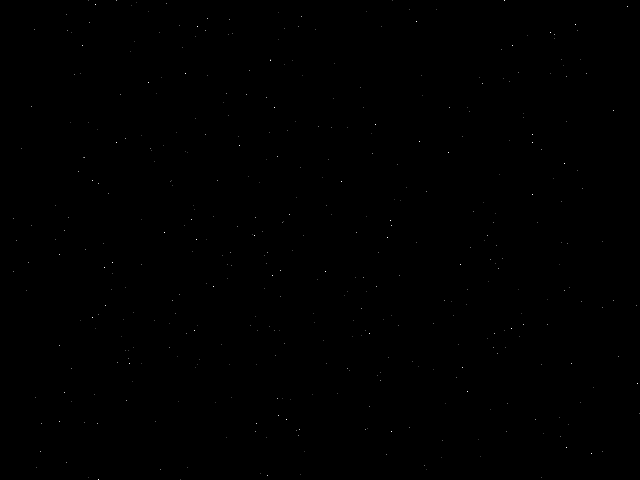
\includegraphics[width=0.7\linewidth]{screenshot3.png}
	\caption{Starfield with stars fading}
	\label{fig3}
\end{figure}
\begin{figure}[h!]
	\centering
	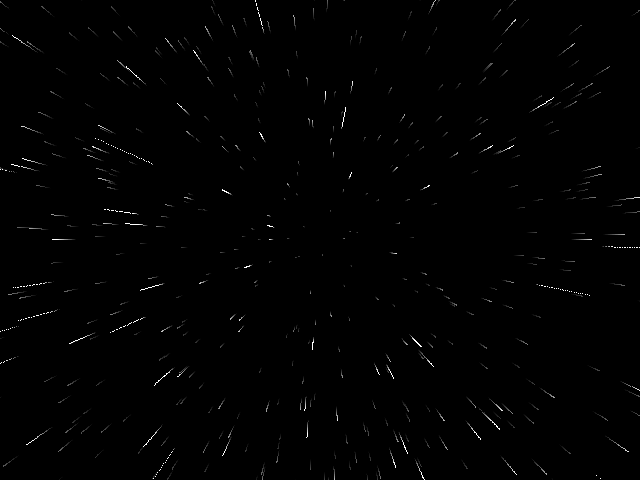
\includegraphics[width=0.7\linewidth]{screenshot4.png}
	\caption{Final output: fading-effect and star-tails.}
	\label{fig4}
\end{figure}


\end{document}
